\documentclass[final,5p,times,twocolumn]{elsarticle}
\usepackage{iftex}\ifPDFTeX\usepackage[T1]{fontenc}\usepackage[utf8]{inputenc}\usepackage{textcomp}\renewcommand{\ttdefault}{lmtt}\else\usepackage{fontspec}\setmainfont{TeX Gyre Termes}\fi
\usepackage{newunicodechar}\newunicodechar{′}{\ensuremath{'}}\newunicodechar{−}{\ensuremath{-}}\newunicodechar{≥}{\ensuremath{\geq}}\newunicodechar{≤}{\ensuremath{\leq}}\newunicodechar{×}{\ensuremath{\times}}\newunicodechar{Δ}{\ensuremath{\Delta}}\newunicodechar{→}{\ensuremath{\rightarrow}}\newunicodechar{Σ}{\ensuremath{\Sigma}}
\usepackage{amsmath,amssymb,graphicx,booktabs,tabularx,array,xurl,needspace}
\makeatletter\def\ps@pprintTitle{\let\@oddhead\@empty\let\@evenhead\@empty\let\@oddfoot\@empty\let\@evenfoot\@oddfoot}\makeatother
\usepackage[hidelinks]{hyperref}\usepackage{orcidlink}
\providecommand{\tightlist}{\setlength{\itemsep}{0pt}\setlength{\parskip}{0pt}}
\setlength{\emergencystretch}{3em}

\journal{International Journal of Medical Informatics}
\begin{document}
\begin{frontmatter}
\title{Attribution is not mitigation: a paired-label counterfactual audit of hypertension classification models}
\author[uit,vnu]{Cong-Danh Tran}
\makeatletter\g@addto@macro\elsauthors{\,\orcidlink{0009-0001-9660-8808}}\makeatother
\ead{danhtc@grad.uit.edu.vn}
\affiliation[uit]{organization={University of Information Technology}, city={Ho Chi Minh City}, country={Viet Nam}}
\affiliation[vnu]{organization={Vietnam National University}, city={Ho Chi Minh City}, country={Viet Nam}}
\begin{abstract}
\textbf{Background:} Counterfactual explanations (CFs) show which input changes would change a model's prediction. A hypertension label based on self-reported diagnosis reflects both the disease and whether it has been diagnosed. It is unclear how this affects CFs, and whether restricting CF changes removes the effect.

\textbf{Objective:} To test separately how much models rely on each feature group, how much a group contributes to the difference between two models' responses to the same CF, and whether locking that group in new CFs reduces this difference.

\textbf{Methods:} In the National Health and Nutrition Examination Survey (NHANES), each adult has a self-reported label and an examination-based label (blood pressure ≥140/90 mmHg [18.7/12.0 kPa] or treatment). XGBoost models differed only in their training label. We measured grouped permutation importance, generated CFs with DiCE, scored each CF with one evaluation model per label, reset diagnosis-related features in generated CFs (ablation), and generated new CFs with these features locked or under guideline-based rules. The procedure was developed on 2011–2014 data (n = 10,311) and applied to 2015–2018 data (n = 10,151) with retrained models.

\textbf{Results:} In 2015–2018, permuting access-to-care features reduced the area under the ROC curve (AUC) more for the self-report model (difference 0.014 [0.008; 0.019]); this was not reproduced with a blood-pressure-only label in untreated adults. Diagnosis-related changes contributed 4.3 percentile points (lower bound 3.7; 2015–2018, primary seed) to the difference in score drops between the evaluation models; this contribution was positive in all seeds and both periods. Ablation reduced this difference by 50–67\%; locking reduced it by 9–27\% and was unstable in 2011–2014. Under guideline-based rules, only 3–12\% of individuals had a valid CF.

\textbf{Conclusion:} Knowing which features contribute to a difference does not show that locking them will reduce it.
\end{abstract}

\begin{keyword}
Counterfactual explanations \sep Explainable artificial intelligence \sep Clinical decision support \sep Label bias \sep Hypertension \sep NHANES
\end{keyword}
\end{frontmatter}
\section{Introduction}

Counterfactual explanations (CFs) describe small changes to a person's
features that would change a model's prediction {[}1,2{]}. In clinical
decision support {[}3{]}, a CF may be shown as a suggestion, such as
reducing waist circumference, although it only shows what would change
one model's output, not what would improve health {[}4,5{]}.

A model learns whatever its training label records. Many people with
hypertension are undiagnosed {[}6,7{]}, so self-report misses cases
found by measurement {[}8{]}. The way an outcome is recorded can bias
predictions {[}9--11{]}. For a model trained on self-reported diagnosis,
insurance or a usual place of care can predict who has been diagnosed
rather than blood pressure, and its CFs may then suggest changing them.

Thieu {[}12{]} proposed a directional taxonomy that restricts how each
feature may change in diabetes CFs, and suggested that some implausible
CFs may come from self-reported labels; the data had no measured label
for comparison. Changing a label definition changes the resulting CFs
{[}13{]}, as does changing among models of similar accuracy {[}14,15{]}.
What is still missing is a test, on the same people, of how much a
feature group contributes to the difference between two clinical label
definitions, and whether restricting that group reduces it. This matters
because the usual response to an implausible CF is to lock the feature
involved {[}12,16,17{]}.

We propose the Paired-Label Counterfactual Audit (PLCA), an audit
procedure based on two label definitions recorded for the same people.
The National Health and Nutrition Examination Survey (NHANES) suits this
design because participants report whether they have ever been told that
they have hypertension, and their blood pressure is measured in the same
survey. PLCA asks three questions: (1) \emph{reliance}: does the
self-report model need access-to-care features more? (2)
\emph{contribution}: how much do diagnosis-related changes contribute to
the difference between the two models' responses to the same CF? (3)
\emph{mitigation}: does locking these features reduce the difference,
and can valid CFs still be found under guideline-based rules?

PLCA separates the contribution of a feature group in generated CFs (E2)
from the effect of locking it in new CFs (E3). It is not a new CF
algorithm or importance method; it combines existing analyses on two
clinical labels for the same people.

\section{Methods}

\subsection{Data and labels}

We used public NHANES data {[}18,19{]}. The procedure was developed on
2011--2014 data (n = 10,311) and applied to 2015--2018 data (n = 10,151)
with all models retrained. We included non-pregnant adults aged ≥20
years with valid blood pressure readings, an answer to BPQ020, and known
treatment status.

Each person had two labels. \emph{\(Y_{\mathrm{self}}\)} was 1 if the
person had ever been told by a doctor or other health professional that
they had hypertension. \emph{\(Y_{\mathrm{clin}}\)}, the
examination-based label, was 1 if systolic pressure was ≥140 mmHg (18.7
kPa), diastolic pressure was ≥90 mmHg (12.0 kPa), or the person was
taking blood pressure medication. The 130/80 mmHg (17.3/10.7 kPa)
threshold {[}6{]} was a sensitivity analysis. People without a reported
diagnosis are not asked about treatment and were coded as untreated.
\(Y_{\mathrm{clin}}\) is a phenotype, not ground truth, and its
treatment component still depends on past diagnosis. Pairs
(\(Y_{\mathrm{self}}\), \(Y_{\mathrm{clin}}\)) define four groups: G00,
G01 (examination-positive only), G10 (self-report-positive only) and
G11. Fig. 1 summarizes the design.

\begin{figure*}[!htbp]\centering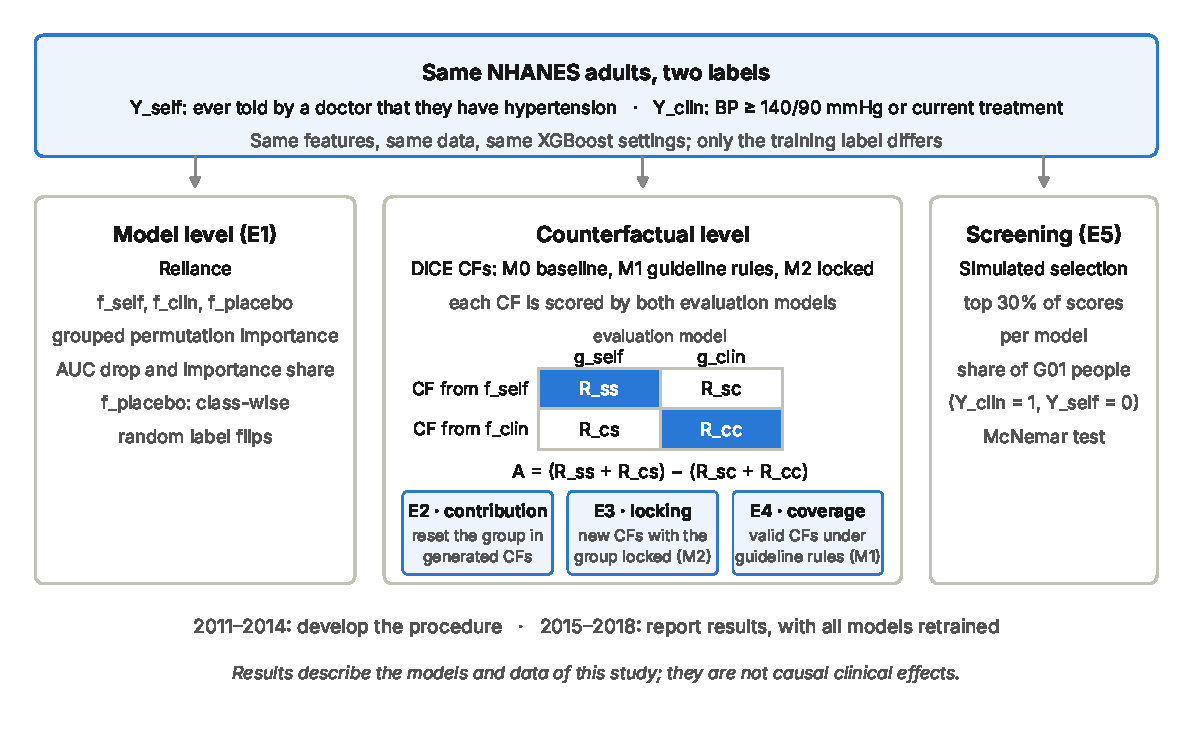
\includegraphics[width=\textwidth]{fig1.pdf}\caption{Design of PLCA. The models differ only in the training label. At the CF level, each CF is scored by both evaluation models, which gives a 2 × 2 same-label and cross-label matrix (dark cells: same label). E2 analyses generated CFs; E3 generates new CFs with the group locked.}\end{figure*}

\subsection{Features and preprocessing}

Models used six feature groups: demographics and socioeconomic status;
access to care (insurance, usual place of care, health care visits);
other diagnoses (diabetes, high cholesterol); lifestyle (smoking, drinks
per drinking day, moderate and vigorous recreational activity);
physiology (body mass index (BMI), waist, total cholesterol, HbA1c); and
self-rated health. Sex was the sex recorded by NHANES; gender was not
available. Blood pressure measurements and blood pressure questions were
not inputs. ``Cholesterol ever checked'' (BPQ060) was excluded because
its missingness depends on \(Y_{\mathrm{self}}\) through skip patterns
(57.8\% vs 26.0\%). We call access to care, other diagnoses and
self-rated health together the \emph{diagnosis-related features}. Data
were split before preprocessing. For E1, XGBoost handled missing values
natively; for CF analyses, missing values were filled with the
training-split median. The feature dictionary, distributions and
missingness are given in the supplementary material (Appendix A).

\subsection{Reliance (E1)}

XGBoost {[}20{]} models (300 trees, depth 4, learning rate 0.05, row and
column subsampling 0.8; fixed in advance, not tuned) were trained on a
70/30 split stratified by \(Y_{\mathrm{clin}}\).
\emph{\(f_{\mathrm{self}}\)} learned \(Y_{\mathrm{self}}\) and
\emph{\(f_{\mathrm{clin}}\)} learned \(Y_{\mathrm{clin}}\). A
label-noise control, \emph{\(f_{\mathrm{placebo}}\)}, learned
\(Y_{\mathrm{clin}}\) after random flips whose rates depended only on
the \(Y_{\mathrm{clin}}\) class and matched the observed disagreement in
the training data. Grouped permutation importance {[}21--23{]} permuted
all features in a group together on the test set and recorded the AUC
(area under the receiver operating characteristic curve) drop (mean of
three permutations). Shares divided each group's positive importance by
the sum over groups. A two-level bootstrap (B = 100) resampled both the
training set (models retrained) and the test set {[}24{]}. E1 required
the 2.5th percentile of the AUC-drop difference \(f_{\mathrm{self}}\) −
\(f_{\mathrm{clin}}\) for access to care to be above 0, and a positive
mean difference in importance share between \(f_{\mathrm{self}}\) and
\(f_{\mathrm{placebo}}\); the share contrast was interpretable only if
the share was defined in at least 80\% of bootstrap draws.

\subsection{Counterfactuals and evaluation models}

We selected up to 200 untreated test-set people whom both
\(f_{\mathrm{self}}\) and \(f_{\mathrm{clin}}\) predicted as positive
(probability ≥0.5), ranked by the mean percentile score of the two
models. DiCE 0.12 {[}2{]} (random search) was asked for up to five CFs
per person in each constraint mode (Table 1). A CF was \emph{valid} if
it obeyed the rules of its mode and changed the prediction of the model
that generated it from positive to negative. \emph{Valid-CF coverage}
was the share of selected people with at least one valid CF.

\begin{table*}[!htbp]
\caption{Constraint modes used to generate CFs.}
\label{tab1}
\footnotesize\def\baselinestretch{1}\selectfont\renewcommand{\arraystretch}{1.1}
\begin{tabularx}{\textwidth}{>{\raggedright\arraybackslash}p{0.18\linewidth}>{\raggedright\arraybackslash}X>{\raggedright\arraybackslash}X}
\toprule
\textbf{Mode} & \textbf{What DiCE may change} & \textbf{Purpose} \\ \midrule
M0, baseline & Everything except age, sex and race/ethnicity & Reference \\
M1, guideline-based rules & Eight features, only in the guideline direction (Appendix Table A.4); everything else fixed & Can valid CFs be found under clinically motivated rules? \\
M2, locking & As M0, with access to care, other diagnoses and self-rated health fixed & Does locking diagnosis-related features reduce the difference? \\
\bottomrule
\end{tabularx}
\end{table*}

Under M1, BMI and waist may fall only to their thresholds (25 kg/m², or
23 for non-Hispanic Asian people; 102 cm for men, 88 cm for women)
{[}25--29{]}; imputed values are fixed (Appendix Table A.4).

We trained one \emph{evaluation model} per label, \(g_{\mathrm{self}}\)
and \(g_{\mathrm{clin}}\), on the same bootstrap sample of the training
set, and scored every CF with both. Because the two models have
different score distributions, scores were converted to percentiles:
\(p_m(x)\) is the share of test-set people whose \(g_m\) score is not
higher than that of x. The \emph{score drop} of a CF \(x'\) for person x
is

\[\Delta_m(x') = p_m(x) - p_m(x').\]

Let \(R_{sm}\) be the mean drop on evaluation model m for CFs generated
by model s (first averaged over the CFs of each person, then over
people). We define

\[\mathrm{ECD}_{\mathrm{self}} = R_{ss} - R_{sc}, \qquad \mathrm{ECD}_{\mathrm{clin}} = R_{cc} - R_{cs},\]

\[A = \mathrm{ECD}_{\mathrm{self}} - \mathrm{ECD}_{\mathrm{clin}} = (R_{ss}+R_{cs}) - (R_{sc}+R_{cc}).\]

\emph{A/2 is the difference between the mean score drops of
\(g_{\mathrm{self}}\) and \(g_{\mathrm{clin}}\)}, with both CF sources
weighted equally; A \textgreater{} 0 means that \(g_{\mathrm{self}}\)
drops more. These quantities say nothing about real hypertension risk.

\subsection{Contribution (E2) and locking (E3)}

\emph{E2} uses the valid CFs generated under M0. For each CF \(x'\), we
built \(x'_{\mathrm{abl}}\) by resetting all diagnosis-related features
to the person's original values, keeping every other change
(\emph{ablation}). The score recovered on model m is \(C_m\) =
\(p_m(x'_{\mathrm{abl}})\) − \(p_m(x')\), and

\[\mathrm{E2} = \overline{C_{\mathrm{self}} - C_{\mathrm{clin}}} = \tfrac{1}{2}\left[A(\mathrm{M0}) - A_{\mathrm{abl}}\right],\]

averaged per person, with equal weight for the two CF sources; the
ablated CF need not stay valid. E2 was computed on S0, the people with
at least one valid CF from both models under M0.

\emph{E3} asks DiCE for new CFs under M2. On S02, the people in S0 who
also had valid CFs from both models under M2, E3 required

\[A(\mathrm{M0}) > 0 \quad \text{and} \quad |A(\mathrm{M2})| < |A(\mathrm{M0})|.\]

A change of sign with a larger size does not count. When A(M0)
\textgreater{} 0, this is equivalent to A(M0) − A(M2) \textgreater{} 0
and A(M0) + A(M2) \textgreater{} 0. For a descriptive comparison,
\(A_{\mathrm{abl}}\) was also computed on S02, and the reduction in
\textbar A\textbar{} was 100·(\textbar A(M0)\textbar{} −
\textbar{}\(A_{\mathrm{after}}\)\textbar)/\textbar A(M0)\textbar.

\emph{E4} reported valid-CF coverage under M1 and the change in
\(\mathrm{ECD}_{self}\) from M0 to M1, the latter only when at least 40
people had valid CFs from \(f_{\mathrm{self}}\) in both modes.

\subsection{Statistical analysis}

E3 used a participant-level bootstrap (B = 5,000); each inequality was
tested with the one-sided 2.5th percentile, and all had to hold
(intersection--union test). E2 was secondary and used the same
bootstrap. No correction for multiple endpoints was applied. Analyses
required at least 80 eligible people and 40 people in the analysis set.
CF analyses were run with seeds 42 (primary), 43 and 44; for E2 and E3,
seed 42 decided and the other seeds had to give point estimates in the
same direction. Seeds are not independent replications. The bootstrap
intervals are conditional on the trained models and on the people with
valid CFs. \emph{E5}, a secondary screening analysis, compared the share
of G01 people in the top 30\% of scores of each model with an exact
McNemar test {[}30{]}. Table 2 used survey weights and Taylor
linearization {[}19{]}; the models did not use weights. As a post hoc
reporting analysis, we refitted the audited models and report test-set
discrimination, threshold metrics at 0.5 and calibration (Appendix A).
The study was not registered and follows TRIPOD+AI {[}31{]}.

\subsection{Sensitivity analyses and reproducibility}

Sensitivity analyses (seed 42) changed the label definitions, the cycle,
the model, the CF search and the selected people (Table 5). M2-phys
locked physiology instead of diagnosis-related features, and M3 added a
maximum 5\% reduction in BMI and waist to M1. All results come from one
run of \url{scripts/run_all.sh} (software and hardware: Appendix A).

\section{Results}

\subsection{Sample}

In 2015--2018, the two labels disagreed for a survey-weighted 12.9\%
{[}11.8; 13.9{]} of adults (23.1\% {[}21.8; 24.3{]} with 130/80 mmHg).
Compared with G11, G01 people were less likely to have a usual place of
care or a visit in the past year (Table 2). The models used for CFs had
test AUROC 0.810 (\(f_{\mathrm{self}}\)) and 0.836
(\(f_{\mathrm{clin}}\)) in 2015--2018, with balanced accuracy 0.726 and
0.752 at threshold 0.5 and calibration slopes 0.82 and 0.86 (Appendix
Table A.7).

\begin{table*}[!htbp]
\caption{Characteristics of the 2015–2018 sample by label pair (140/90 mmHg).}
\label{tab2}
\footnotesize\def\baselinestretch{1}\selectfont\renewcommand{\arraystretch}{1.1}
\begin{tabularx}{\textwidth}{>{\raggedright\arraybackslash}p{0.24\linewidth}>{\raggedright\arraybackslash}X>{\raggedright\arraybackslash}X>{\raggedright\arraybackslash}X>{\raggedright\arraybackslash}X>{\raggedright\arraybackslash}X}
\toprule
\textbf{Characteristic} & \textbf{All} & \textbf{G00} & \textbf{G01} & \textbf{G10} & \textbf{G11} \\ \midrule
People (unweighted) & 10,151 & 5,533 & 785 & 562 & 3,271 \\
Age, years, mean (SD) & 48.4 (17.2) & 42.1 (15.6) & 56.4 (15.3) & 44.5 (15.5) & 61.2 (13.0) \\
Women, \% & 51.1 & 52.3 & 45.3 & 41.7 & 51.9 \\
Non-Hispanic Black, \% & 11.3 & 9.7 & 12.1 & 10.9 & 14.7 \\
College graduate or above, \% & 31.6 & 35.4 & 30.3 & 28.4 & 24.3 \\
Income-to-poverty ratio < 1.3, \% & 20.3 & 19.8 & 20.5 & 25.5 & 20.1 \\
Insured, \% & 86.5 & 84.0 [81.2; 86.8] & 88.8 [85.2; 92.5] & 82.4 [77.2; 87.6] & 92.5 [90.4; 94.5] \\
Usual place of care, \% & 82.6 & 78.0 [75.8; 80.1] & 81.8 [77.9; 85.7] & 78.7 [72.5; 84.8] & 93.9 [92.6; 95.2] \\
Visit in past year, \% & 83.9 & 79.1 [77.5; 80.7] & 78.8 [74.5; 83.0] & 82.2 [78.4; 86.0] & 96.2 [95.3; 97.0] \\
BMI, kg/m², mean (SD) & 29.6 (7.1) & 28.3 (6.7) & 30.3 (7.3) & 30.9 (7.4) & 32.0 (7.2) \\
Systolic BP, mmHg, mean (SD) & 123.7 (17.7) & 115.8 (10.8) & 148.2 (13.1) & 122.0 (9.7) & 135.3 (20.0) \\
On BP medication, \% & 24.1 & 0 & 0 & 0 & 89.2 \\
\bottomrule
\end{tabularx}
\par\vspace{2pt}{\scriptsize\raggedright G00: both labels 0; G01: $Y_{\mathrm{clin}}$ = 1, $Y_{\mathrm{self}}$ = 0; G10: $Y_{\mathrm{self}}$ = 1, $Y_{\mathrm{clin}}$ = 0; G11: both 1. Survey-weighted (WTMEC2YR divided by the number of cycles); 95\% confidence intervals for access-to-care rows by Taylor linearization. Medication is 0 outside G11 by label definition and skip pattern. Full table: Appendix Table A.6.\par}
\end{table*}

\subsection{Reliance (E1)}

Test-set AUC (mean over bootstrap refits) was 0.806 for
\(f_{\mathrm{self}}\) and 0.831 for \(f_{\mathrm{clin}}\). Permuting
access-to-care features reduced the AUC of \(f_{\mathrm{self}}\) more
than that of \(f_{\mathrm{clin}}\) by 0.014 {[}0.008; 0.019{]} (Fig. 2).
The importance share of access to care was 9.8\% in
\(f_{\mathrm{self}}\) and 2.8\% in \(f_{\mathrm{placebo}}\) (difference
7.0 percentage points {[}2.4; 11.0{]}), so class-wise random label noise
did not reproduce this reliance. The result was similar in 2011--2014
(0.015 {[}0.009; 0.022{]}). Removing G01 people from training reduced it
to 0.005 {[}0.000; 0.010{]} (random removal: 0.014).

An important limit: in untreated people, compared with a
blood-pressure-only label, the difference was −0.003 {[}−0.017;
0.011{]}. E1 therefore depends on the phenotype definition and the
population.

\begin{figure}[!htbp]\centering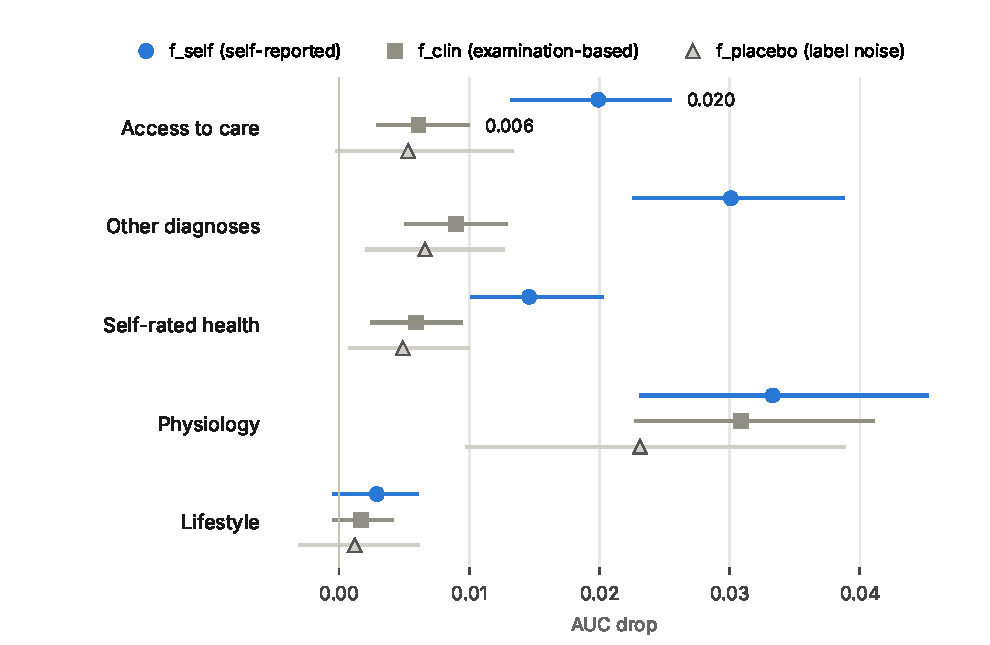
\includegraphics[width=\columnwidth]{fig2.pdf}\caption{AUC drop when each feature group is permuted, for the three models (NHANES 2015–2018, seed 42, two-level bootstrap B = 100). Dots are estimates and lines are 95\% intervals. Demographics are not shown ($f_{\mathrm{self}}$ 0.103; $f_{\mathrm{clin}}$ 0.211).}\end{figure}

\subsection{Contribution (E2)}

Resetting diagnosis-related features in M0 CFs raised the percentile
score of \(g_{\mathrm{self}}\) more than that of \(g_{\mathrm{clin}}\)
by 4.3 percentile points (E2 = 0.043; lower bound 0.037; n = 187). E2
was 0.044 (0.037) and 0.058 (0.049) in seeds 43 and 44, and positive in
all three seeds of 2011--2014 (Appendix Table A.5). It was positive for
CFs from both \(f_{\mathrm{self}}\) (0.057) and \(f_{\mathrm{clin}}\)
(0.030). Between 49\% and 65\% of valid M0 CFs changed at least one
diagnosis-related feature. Access to care, other diagnoses and
self-rated health each contributed, but their order changed between
seeds (Table 4).

\subsection{Locking (E3)}

In seed 42, 172 people formed S02. A(M0) was 0.120 (lower bound 0.097).
With diagnosis-related features locked, A(M2) was 0.087; A(M0) − A(M2)
was 0.033 (0.012) and A(M0) + A(M2) had a lower bound of 0.160, so E3
was met (Table 3). In seeds 43 and 44, all point estimates were
positive, but the lower bound of A(M0) − A(M2) was negative (−0.009 and
−0.004). When all returned CFs were used, including invalid ones, E3 was
not met in any seed. In 2011--2014, E3 was not met: A changed sign under
M2 in seeds 42 and 43, and the change in \textbar A\textbar{} ranged
from a 51\% fall to a 26\% rise (Appendix Table A.5).

On the same S02 sets in 2015--2018, ablation reduced
\textbar A\textbar{} by 64\%, 67\% and 50\%, while locking reduced it by
27\%, 24\% and 9\% (Fig. 3). This is descriptive: ablation edits
existing CFs, whereas locking generates new ones.

\begin{figure}[!htbp]\centering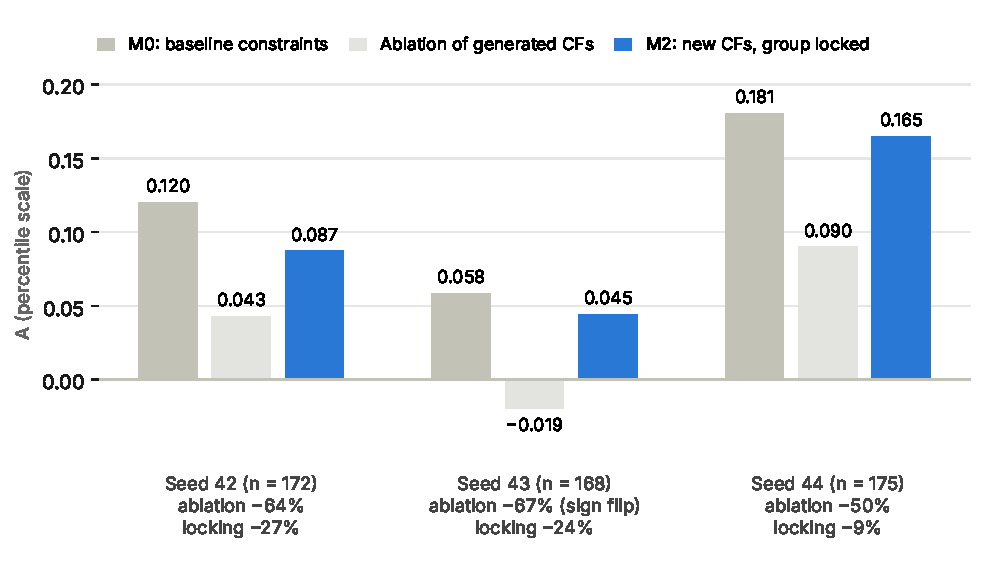
\includegraphics[width=\columnwidth]{fig3.pdf}\caption{A under M0, after ablation and under M2 (locking), on the same people (S02) in each seed, NHANES 2015–2018. Reductions are in |A|. In seed 43, A changes sign after ablation.}\end{figure}

\begin{table*}[!htbp]
\caption{Main results, NHANES 2015–2018. Lower bounds (2.5th percentile, participant-level bootstrap, B = 5,000) in parentheses; 95\% intervals (two-level bootstrap, B = 100) in brackets.}
\label{tab3}
\footnotesize\def\baselinestretch{1}\selectfont\renewcommand{\arraystretch}{1.1}
\begin{tabularx}{\textwidth}{>{\raggedright\arraybackslash}p{0.10\linewidth}>{\raggedright\arraybackslash}X>{\raggedright\arraybackslash}X>{\raggedright\arraybackslash}X>{\raggedright\arraybackslash}X>{\raggedright\arraybackslash}X}
\toprule
\textbf{Endpoint} & \textbf{Quantity} & \textbf{Seed 42} & \textbf{Seed 43} & \textbf{Seed 44} & \textbf{Conclusion} \\ \midrule
E1 (primary) & Access-to-care AUC drop, $f_{\mathrm{self}}$ − $f_{\mathrm{clin}}$ & 0.014 [0.008; 0.019] & — & — & Met \\
E2 (secondary) & Contribution of diagnosis-related features, S0 & 0.043 (0.037); n = 187 & 0.044 (0.037); n = 184 & 0.058 (0.049); n = 197 & Met in all seeds \\
E3 (primary) & A(M0); A(M0) − A(M2); A(M0) + A(M2), S02 & 0.120 (0.097); 0.033 (0.012); 0.208 (0.160); n = 172 & 0.058 (0.028); 0.014 (−0.009); 0.103 (0.042); n = 168 & 0.181 (0.156); 0.016 (−0.004); 0.346 (0.300); n = 175 & Met in seed 42; same direction in 43, 44 \\
E4 (descriptive) & Valid-CF coverage from $f_{\mathrm{self}}$, M1 vs M0 & 9.0\% vs 100\%; 18 common & 12.0\% vs 99.5\%; 24 common & 10.5\% vs 99.5\%; 21 common & ECD not interpretable (n < 40) \\
E5 (secondary) & G01 share in top 30\%, $f_{\mathrm{self}}$ vs $f_{\mathrm{clin}}$ & 27.8\% vs 33.3\%; p = 0.029 & — & — & Met pooled; not met per cycle \\
\bottomrule
\end{tabularx}
\end{table*}

\begin{table}[!htbp]
\caption{Contribution of each diagnosis-related group when reset alone, seed 42.}
\label{tab4}
\footnotesize\def\baselinestretch{1}\selectfont\renewcommand{\arraystretch}{1.1}
\begin{tabularx}{\columnwidth}{>{\raggedright\arraybackslash}X>{\raggedright\arraybackslash}X}
\toprule
\textbf{Group} & \textbf{Contribution} \\ \midrule
Access to care & 0.020 \\
Other diagnoses & 0.017 \\
Self-rated health & 0.007 \\
\bottomrule
\end{tabularx}
\par\vspace{2pt}{\scriptsize\raggedright Values do not add up to E2 because features can interact. The largest group was self-rated health in seed 43 (0.022) and other diagnoses in seed 44 (0.031).\par}
\end{table}

\subsection{Guideline-based rules (E4)}

Under M1, DiCE found a valid CF for 9.0--12.0\% of people with
\(f_{\mathrm{self}}\) and 3.0--7.5\% with \(f_{\mathrm{clin}}\),
compared with 92--100\% under M0 and 86--99\% under M2 (Fig. 4). In
88--97\% of failures DiCE returned no CF. Only 18--24 people had valid
\(f_{\mathrm{self}}\) CFs in both M0 and M1 (threshold 40), so we draw
no conclusion on whether the rules reduce the difference. All valid M1
CFs lowered BMI or waist, often by a large amount: the mean relative BMI
reduction was 26--37\%, and 74--94\% of valid CFs reduced BMI by more
than 10\%. No valid M1 CF in 2015--2018 changed access to care, although
the rules allowed it. Coverage was also low in 2011--2014 (8.5--18.0\%
with \(f_{\mathrm{self}}\)). When BMI and waist reductions were limited
to 5\% (M3), coverage fell to 0.5\% (\(f_{\mathrm{self}}\)) and 0\%
(\(f_{\mathrm{clin}}\)).

\begin{figure}[!htbp]\centering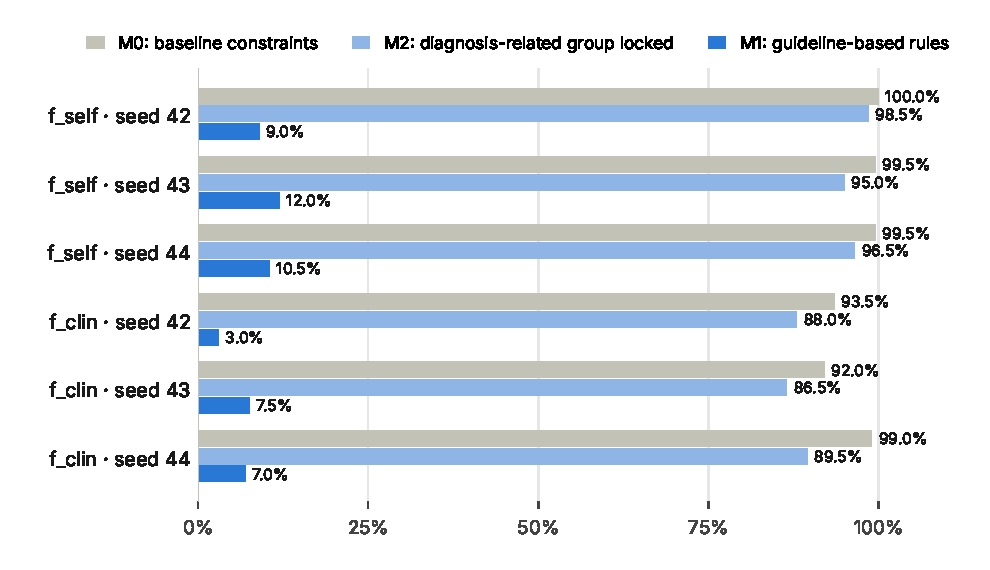
\includegraphics[width=\columnwidth]{fig4.pdf}\caption{Share of the 200 selected people with at least one valid CF under M0 (baseline), M2 (diagnosis-related group locked) and M1 (guideline-based rules), by CF model and seed (NHANES 2015–2018).}\end{figure}

\subsection{Screening (E5) and sensitivity analyses}

In the top 30\% of scores, \(f_{\mathrm{self}}\) selected 27.8\% of G01
people and \(f_{\mathrm{clin}}\) 33.3\% (11 vs 25 discordant people;
exact McNemar p = 0.029), but not significantly within each cycle (p =
0.21 and 0.115). Because G01 is partly defined by \(Y_{\mathrm{clin}}\),
E5 shows different selections, not clinical benefit.

E1 was met in all sensitivity analyses except the blood-pressure-only
label in untreated people, and E3 was met at seed 42 in all three CF
sensitivity analyses (Table 5). With DiCE genetic, A fell from 0.242 to
0.169 (about 30\%), so the size of A depends on the CF algorithm.
Locking physiology instead (M2-phys) increased A from 0.137 to 0.191 on
89 common people, whereas M2 reduced it on the same people (A(M0) −
A(M2) = 0.032 {[}0.003; 0.062{]}).

\begin{table}[!htbp]
\caption{Sensitivity analyses, NHANES 2015–2018, seed 42.}
\label{tab5}
\footnotesize\def\baselinestretch{1}\selectfont\renewcommand{\arraystretch}{1.1}
\begin{tabularx}{\columnwidth}{>{\raggedright\arraybackslash}p{0.40\linewidth}>{\raggedright\arraybackslash}X>{\raggedright\arraybackslash}X>{\raggedright\arraybackslash}X}
\toprule
\textbf{Change} & \textbf{E1} & \textbf{E2} & \textbf{E3} \\ \midrule
130/80 mmHg threshold & 0.019; met & — & — \\
Self-report told ≥2 times & 0.017; met & — & — \\
Reconstructed cholesterol-check variable & 0.016; met & — & — \\
Cycle 2015–2016 / 2017–2018 & 0.011 / 0.015; met & — & — \\
$f_{\mathrm{self}}$ vs blood-pressure-only label, untreated & −0.003; not met & — & — \\
Logistic regression & 0.008; met & 0.085 (n = 191) & Met (n = 88) \\
DiCE genetic & — & 0.105 (n = 192) & Met (n = 177) \\
$Y_{\mathrm{clin}}$ = 1 people only & — & 0.033 (n = 109) & Met (n = 104) \\
All returned CFs & — & — & Not met \\
\bottomrule
\end{tabularx}
\end{table}

\section{Discussion}

\subsection{Main findings}

First, reliance (E1) and contribution (E2) are different estimands; both
pointed in the same direction, but E1 was not reproduced with a
blood-pressure-only label.

Second, knowing the contribution of a group does not tell us what
happens when the group is locked. In 2015--2018, ablation reduced
\textbar A\textbar{} by 50--67\% and locking by only 9--27\%; in
2011--2014, the effect of locking was unstable in both size and sign.
One possible explanation, which we did not test, is that DiCE replaces
the locked features with other changes that still affect the two models
differently. The practical lesson is to measure the result of
constrained CF generation directly, instead of inferring it from
attribution.

Third, following clinical directions does not guarantee that valid CFs
can be found. The guideline-based rules left valid CFs for about one in
ten selected people, and the remaining CFs often required large BMI
reductions. A rule on direction does not limit the size of a change, and
adding a size limit (M3) left almost no CFs. Finding no CF does not
prove that none exists; coverage depends on the algorithm, search budget
and models.

\subsection{Implications and clinical translation roadmap}

Before CFs are shown to clinicians or patients, developers should check
whether the label also records access to diagnosis, report valid-CF
coverage for each constraint setting, and test constraints directly.
Changing a recorded diagnosis or self-rated health in a CF is not an
intervention.

PLCA could serve as a pre-deployment audit step, not a clinical tool:
its intended users are developers and governance teams validating a
CF-based decision support model before release. It is a proof of concept
on survey data (self-assessed technology readiness level 3--4 {[}32{]}).
A proposed path is: (i) rerun PLCA on electronic health record data
where a diagnosis code and measured blood pressure exist for the same
patients; (ii) have clinicians review the constraint rules and a sample
of CFs; (iii) repeat the audit when the model or data change. Whether
this improves clinical decisions or patient outcomes has not been
studied (Appendix A).

\subsection{Relation to previous work}

Thieu {[}12{]} designed rules for how CFs may change and suggested,
without a measured comparison label, that self-reported labels may cause
implausible CFs. PLCA addresses a different question: it uses two labels
for the same people to measure how the label definition affects CF
behavior and whether locking features removes this effect. Our results
are consistent with that suggestion in another disease, but we did not
test the original diabetes taxonomy. Attribution and CFs are known to
disagree {[}33{]}.

\subsection{Limitations}

NHANES is cross-sectional, and the labels differ in timing as well as
recording, so not every disagreement reflects access to care. Results
cover one condition, one country and one CF framework (DiCE, mainly
random search), with one evaluation model per label; other equivalent
models could give different results. The two periods test whether the
procedure can be repeated with retrained models; they are not an
external validation of the classifiers. The CF bootstrap does not
include variation from retraining or CF search. E3 was met only in
2015--2018, and E5 only in pooled data. Because the self-report label
partly reflects access to diagnosis, models trained on it may be less
accurate for groups with less access to care; we did not evaluate
performance by sex or race/ethnicity. The guideline-based rules were not
reviewed by clinicians and cannot represent sodium, potassium, the DASH
diet or stress management. E2 was added during the development phase
after E3 failed in a trial analysis; its definition and role were fixed
before it was computed on 2015--2018 data. E4 is descriptive.

\section{Conclusion}

In NHANES, models trained on two hypertension labels for the same people
relied on different features and responded differently to the same CFs.
Diagnosis-related features contributed to this difference in both survey
periods, but locking them in new CFs did not reduce it consistently, and
guideline-based rules left valid CFs for very few people. Knowing which
features contribute to a difference does not show that restricting them
will fix it. CFs are not treatment advice.


\needspace{16\baselineskip}\section*{Summary table}
\textbf{What was already known on the topic}

\begin{itemize}
\tightlist
\item
  Self-reported hypertension misses undiagnosed cases, so a model
  trained on it can learn who has been diagnosed as well as who has the
  disease.
\item
  Implausible counterfactual suggestions are usually handled by locking
  features or by applying domain-knowledge rules.
\end{itemize}

\textbf{What this study added to our knowledge}

\begin{itemize}
\tightlist
\item
  With two labels for the same NHANES adults, diagnosis-related features
  contributed to how differently two models responded to the same
  counterfactual in both survey periods.
\item
  Locking these features did not reduce the difference consistently, and
  guideline-based rules left valid counterfactuals for only 3--12\% of
  people, so constraints should be tested directly before
  counterfactuals are used in decision support.
\end{itemize}

\section*{CRediT authorship contribution statement}

Cong-Danh Tran: Conceptualization, Methodology, Software, Validation,
Formal analysis, Data curation, Visualization, Writing -- original
draft, Writing -- review \& editing.

\section*{Declaration of competing interest}

The author declares no known competing financial interests or personal
relationships that could have appeared to influence the work reported in
this paper. {[}To be confirmed by the author.{]}

\section*{Funding}

This research did not receive any specific grant from funding agencies
in the public, commercial, or not-for-profit sectors. {[}To be confirmed
by the author.{]}

\section*{Ethics statement}

NHANES protocols were approved by the NCHS Research Ethics Review Board
(Protocol \#2011-17 for 2011--2016, with continuation, and Protocol
\#2018-01 from 26 October 2017), and participants gave written informed
consent. This study is a secondary analysis of the publicly released,
de-identified NHANES files; the author had no access to identifiable
information and no contact with participants. {[}Author to state here
whether institutional review or a formal exemption was obtained; do not
claim an exemption without documentation.{]}

\section*{Data availability}

NHANES data are publicly available from the US National Center for
Health Statistics. Analysis code, run configuration and summary results
are available at https://github.com/danh-tc/plca-hypertension; all
endpoint results were produced by \texttt{scripts/run\_all.sh} at commit
85a813b; the post hoc performance and data-characteristics tables by
\texttt{scripts/run\_posthoc\_performance.sh}. No study protocol was
published, and the study was not registered.

\section*{Patient and public involvement}

Patients and the public were not involved in the design, conduct,
reporting or dissemination of this research.

\section*{Declaration of generative AI and AI-assisted technologies in
the writing process}

During the preparation of this work, the author used Claude (Anthropic)
for language editing, clarity improvement, and assistance with
manuscript preparation and analysis code. All AI-generated output was
reviewed, verified, and edited by the author, who takes full
responsibility for the content of this publication.

\begin{thebibliography}{99}
\bibitem{r1} S. Wachter, B. Mittelstadt, C. Russell, Counterfactual explanations without opening the black box: automated decisions and the GDPR, Harv. J. Law Technol. 31 (2) (2018) 841–887, \url{https://doi.org/10.2139/ssrn.3063289}
\bibitem{r2} R.K. Mothilal, A. Sharma, C. Tan, Explaining machine learning classifiers through diverse counterfactual explanations, in: Proceedings of the 2020 Conference on Fairness, Accountability, and Transparency (FAT*), 2020, pp. 607–617, \url{https://doi.org/10.1145/3351095.3372850}
\bibitem{r3} R.T. Sutton, D. Pincock, D.C. Baumgart, D.C. Sadowski, R.N. Fedorak, K.I. Kroeker, An overview of clinical decision support systems: benefits, risks, and strategies for success, NPJ Digit. Med. 3 (2020) 17, \url{https://doi.org/10.1038/s41746-020-0221-y}
\bibitem{r4} A.-H. Karimi, B. Schölkopf, I. Valera, Algorithmic recourse: from counterfactual explanations to interventions, in: Proceedings of the 2021 ACM Conference on Fairness, Accountability, and Transparency (FAccT '21), 2021, pp. 353–362, \url{https://doi.org/10.1145/3442188.3445899}
\bibitem{r5} S. Barocas, A.D. Selbst, M. Raghavan, The hidden assumptions behind counterfactual explanations and principal reasons, in: Proceedings of the 2020 Conference on Fairness, Accountability, and Transparency (FAT*), 2020, pp. 80–89, \url{https://doi.org/10.1145/3351095.3372830}
\bibitem{r6} P.K. Whelton, R.M. Carey, W.S. Aronow, et al., 2017 ACC/\allowbreak{}AHA/\allowbreak{}AAPA/\allowbreak{}ABC/\allowbreak{}ACPM/\allowbreak{}AGS/\allowbreak{}APhA/\allowbreak{}ASH/\allowbreak{}ASPC/\allowbreak{}NMA/\allowbreak{}PCNA guideline for the prevention, detection, evaluation, and management of high blood pressure in adults, Hypertension 71 (6) (2018) e13–e115, \url{https://doi.org/10.1161/HYP.0000000000000065}
\bibitem{r7} P. Muntner, S.T. Hardy, L.J. Fine, B.C. Jaeger, G. Wozniak, E.B. Levitan, L.D. Colantonio, Trends in blood pressure control among US adults with hypertension, 1999–2000 to 2017–2018, JAMA 324 (12) (2020) 1190–1200, \url{https://doi.org/10.1001/jama.2020.14545}
\bibitem{r8} V.S.S. Gonçalves, K.R.C. Andrade, K.M.B. Carvalho, M.T. Silva, M.G. Pereira, T.F. Galvao, Accuracy of self-reported hypertension: a systematic review and meta-analysis, J. Hypertens. 36 (5) (2018) 970–978, \url{https://doi.org/10.1097/HJH.0000000000001648}
\bibitem{r9} Z. Obermeyer, B. Powers, C. Vogeli, S. Mullainathan, Dissecting racial bias in an algorithm used to manage the health of populations, Science 366 (6464) (2019) 447–453, \url{https://doi.org/10.1126/science.aax2342}
\bibitem{r10} T. Chang, M.W. Sjoding, J. Wiens, Disparate censorship \& undertesting: a source of label bias in clinical machine learning, in: Proceedings of the 7th Machine Learning for Healthcare Conference, PMLR 182, 2022, pp. 343–390
\bibitem{r11} M. Zanger-Tishler, J. Nyarko, S. Goel, Risk scores, label bias, and everything but the kitchen sink, Sci. Adv. 10 (13) (2024) eadi8411, \url{https://doi.org/10.1126/sciadv.adi8411}
\bibitem{r12} V. Thieu, Knowledge-guided counterfactual explanations for diabetes risk decision support: a directional intervention taxonomy, Int. J. Med. Inform. 219 (2026) 106555, \url{https://doi.org/10.1016/j.ijmedinf.2026.106555}
\bibitem{r13} M. Cerrato, O. Sahlgren, X. Heilmann, Taking the whys seriously: limitations of counterfactual explanations in justification and recourse, arXiv preprint arXiv:2608.30956, 2026, \url{https://doi.org/10.48550/arXiv.2608.30956}
\bibitem{r14} M. Pawelczyk, K. Broelemann, G. Kasneci, On counterfactual explanations under predictive multiplicity, in: Proceedings of the 36th Conference on Uncertainty in Artificial Intelligence (UAI), PMLR 124, 2020, pp. 809–818
\bibitem{r15} J. Jiang, F. Leofante, A. Rago, F. Toni, Robust counterfactual explanations in machine learning: a survey, in: Proceedings of the Thirty-Third International Joint Conference on Artificial Intelligence (IJCAI-24), Survey Track, 2024, pp. 8086–8094, \url{https://doi.org/10.24963/ijcai.2024/894}
\bibitem{r16} S. Bobek, Ł. Bałec, G.J. Nalepa, Actionable and diverse counterfactual explanations incorporating domain knowledge and plausibility constraints, arXiv preprint arXiv:2511.20236v3, 2026, \url{https://doi.org/10.48550/arXiv.2511.20236}
\bibitem{r17} R. Poyiadzi, K. Sokol, R. Santos-Rodriguez, T. De Bie, P. Flach, FACE: feasible and actionable counterfactual explanations, in: Proceedings of the 2020 AAAI/\allowbreak{}ACM Conference on AI, Ethics, and Society (AIES '20), 2020, pp. 344–350, \url{https://doi.org/10.1145/3375627.3375850}
\bibitem{r18} National Center for Health Statistics, National Health and Nutrition Examination Survey: analytic guidelines, 2011–2014 and 2015–2016, NCHS, Hyattsville, MD, 2018, \url{https://wwwn.cdc.gov/Nchs/data/nhanes/analyticguidelines/11-16-analytic-guidelines.pdf}
\bibitem{r19} T.C. Chen, J. Clark, M.K. Riddles, L.K. Mohadjer, T.H.I. Fakhouri, National Health and Nutrition Examination Survey, 2015–2018: sample design and estimation procedures, Vital Health Stat. 2 (184) (2020) 1–35
\bibitem{r20} T. Chen, C. Guestrin, XGBoost: a scalable tree boosting system, in: Proceedings of the 22nd ACM SIGKDD International Conference on Knowledge Discovery and Data Mining (KDD '16), 2016, pp. 785–794, \url{https://doi.org/10.1145/2939672.2939785}
\bibitem{r21} L. Breiman, Random forests, Mach. Learn. 45 (1) (2001) 5–32, \url{https://doi.org/10.1023/A:1010933404324}
\bibitem{r22} A. Fisher, C. Rudin, F. Dominici, All models are wrong, but many are useful: learning a variable's importance by studying an entire class of prediction models simultaneously, J. Mach. Learn. Res. 20 (177) (2019) 1–81
\bibitem{r23} Q. Au, J. Herbinger, C. Stachl, B. Bischl, G. Casalicchio, Grouped feature importance and combined features effect plot, Data Min. Knowl. Discov. 36 (4) (2022) 1401–1450, \url{https://doi.org/10.1007/s10618-022-00840-5}
\bibitem{r24} B. Efron, Bootstrap methods: another look at the jackknife, Ann. Stat. 7 (1) (1979) 1–26, \url{https://doi.org/10.1214/aos/1176344552}
\bibitem{r25} D.W. Jones, K.C. Ferdinand, S.J. Taler, et al., 2025 AHA/\allowbreak{}ACC/\allowbreak{}AANP/\allowbreak{}AAPA/\allowbreak{}ABC/\allowbreak{}ACCP/\allowbreak{}ACPM/\allowbreak{}AGS/\allowbreak{}AMA/\allowbreak{}ASPC/\allowbreak{}NMA/\allowbreak{}PCNA/\allowbreak{}SGIM guideline for the prevention, detection, evaluation and management of high blood pressure in adults: a report of the American College of Cardiology/\allowbreak{}American Heart Association Joint Committee on Clinical Practice Guidelines, Circulation 152 (2025) e114–e218, \url{https://doi.org/10.1161/CIR.0000000000001356}
\bibitem{r26} S.M. Grundy, J.I. Cleeman, S.R. Daniels, et al., Diagnosis and management of the metabolic syndrome: an American Heart Association/\allowbreak{}National Heart, Lung, and Blood Institute scientific statement, Circulation 112 (17) (2005) 2735–2752, \url{https://doi.org/10.1161/CIRCULATIONAHA.105.169404}
\bibitem{r27} K.G.M.M. Alberti, R.H. Eckel, S.M. Grundy, et al., Harmonizing the metabolic syndrome: a joint interim statement, Circulation 120 (16) (2009) 1640–1645, \url{https://doi.org/10.1161/CIRCULATIONAHA.109.192644}
\bibitem{r28} R.S. Blumenthal, P.B. Morris, M. Gaudino, et al., 2026 ACC/\allowbreak{}AHA/\allowbreak{}AACVPR/\allowbreak{}ABC/\allowbreak{}ACPM/\allowbreak{}ADA/\allowbreak{}AGS/\allowbreak{}APhA/\allowbreak{}ASPC/\allowbreak{}NLA/\allowbreak{}PCNA guideline on the management of dyslipidemia, J. Am. Coll. Cardiol. (2026), \url{https://doi.org/10.1016/j.jacc.2025.11.016}
\bibitem{r29} F.C. Bull, S.S. Al-Ansari, S. Biddle, et al., World Health Organization 2020 guidelines on physical activity and sedentary behaviour, Br. J. Sports Med. 54 (24) (2020) 1451–1462, \url{https://doi.org/10.1136/bjsports-2020-102955}
\bibitem{r30} Q. McNemar, Note on the sampling error of the difference between correlated proportions or percentages, Psychometrika 12 (2) (1947) 153–157, \url{https://doi.org/10.1007/BF02295996}
\bibitem{r31} G.S. Collins, K.G.M. Moons, P. Dhiman, et al., TRIPOD+AI statement: updated guidance for reporting clinical prediction models that use regression or machine learning methods, BMJ 385 (2024) e078378, \url{https://doi.org/10.1136/bmj-2023-078378}
\bibitem{r32} A. Lavin, C.M. Gilligan-Lee, A. Visnjic, S. Ganju, D. Newman, S. Ganguly, D. Lange, A.G. Baydin, A. Sharma, A. Gibson, S. Zheng, E.P. Xing, C. Mattmann, J. Parr, Y. Gal, Technology readiness levels for machine learning systems, Nat. Commun. 13 (2022) 6039, \url{https://doi.org/10.1038/s41467-022-33128-9}
\bibitem{r33} R.K. Mothilal, D. Mahajan, C. Tan, A. Sharma, Towards unifying feature attribution and counterfactual explanations: different means to the same end, in: Proceedings of the 2021 AAAI/\allowbreak{}ACM Conference on AI, Ethics, and Society (AIES '21), 2021, pp. 652–663, \url{https://doi.org/10.1145/3461702.3462597}
\end{thebibliography}
\clearpage
\appendix
\setcounter{table}{0}\setcounter{figure}{0}
\section{Supplementary material}

\begin{table*}[!htbp]
\caption{Scope of the conclusions.}
\label{tabA1}
\footnotesize\def\baselinestretch{1}\selectfont\renewcommand{\arraystretch}{1.1}
\begin{tabularx}{\textwidth}{>{\raggedright\arraybackslash}X>{\raggedright\arraybackslash}X}
\toprule
\textbf{Supported by the results} & \textbf{Not shown by this study} \\ \midrule
In the main setting, the self-report model relies more on access-to-care features than the examination-based model. & Access to care causes hypertension, or the model is wrong in a causal sense. \\
Class-wise random label noise does not reproduce the reliance of $f_{\mathrm{self}}$ on access to care. & All label-noise mechanisms are ruled out. \\
In generated CFs, diagnosis-related changes contribute to the difference in score drops between the evaluation models. & E2 measures a causal effect or the exact share of shortcut use. \\
Locking the group when new CFs are generated has an unstable effect on |A|; in 2015–2018 it reduced the difference only partly. & The result holds for every CF algorithm or data set. \\
Under the guideline-based rules, DiCE found valid CFs for very few people in the tested setting. & No other valid CF exists, or the rules are clinically validated. \\
A paired-label audit can be run on public NHANES data. & CFs are treatment advice or have been reviewed by clinicians. \\
\bottomrule
\end{tabularx}
\end{table*}

\begin{table*}[!htbp]
\caption{Components of A and I on the same people (S02), NHANES 2015–2018.}
\label{tabA2}
\footnotesize\def\baselinestretch{1}\selectfont\renewcommand{\arraystretch}{1.1}
\begin{tabularx}{\textwidth}{>{\raggedright\arraybackslash}X>{\raggedright\arraybackslash}X>{\raggedright\arraybackslash}X>{\raggedright\arraybackslash}X>{\raggedright\arraybackslash}X>{\raggedright\arraybackslash}X>{\raggedright\arraybackslash}X}
\toprule
\textbf{Seed} & \textbf{Mode} & \textbf{n} & \textbf{$\mathrm{ECD}_{self}$} & \textbf{$\mathrm{ECD}_{clin}$} & \textbf{A} & \textbf{I} \\ \midrule
42 & M0 & 172 & 0.089 & −0.031 & 0.120 & 0.058 \\
42 & M2 & 172 & 0.070 & −0.018 & 0.087 & 0.052 \\
43 & M0 & 168 & 0.073 & 0.015 & 0.058 & 0.088 \\
43 & M2 & 168 & 0.079 & 0.035 & 0.045 & 0.114 \\
44 & M0 & 175 & 0.125 & −0.055 & 0.181 & 0.070 \\
44 & M2 & 175 & 0.154 & −0.010 & 0.165 & 0.144 \\
\bottomrule
\end{tabularx}
\par\vspace{2pt}{\scriptsize\raggedright I = $\mathrm{ECD}_{self}$ + $\mathrm{ECD}_{clin}$; I/2 is the mean difference between the score drop on the same-label and the cross-label evaluation model, with both CF sources weighted equally. I is descriptive and has no interval. Locking reduced A but did not consistently reduce I. Source: \url{results/confirmation/cf_primary/C6_all_seeds.csv}.\par}
\end{table*}

\begin{table*}[!htbp]
\caption{Mean score drop per CF, by CF model and mode, seed 42.}
\label{tabA3}
\footnotesize\def\baselinestretch{1}\selectfont\renewcommand{\arraystretch}{1.1}
\begin{tabularx}{\textwidth}{>{\raggedright\arraybackslash}X>{\raggedright\arraybackslash}X>{\raggedright\arraybackslash}X>{\raggedright\arraybackslash}X>{\raggedright\arraybackslash}X>{\raggedright\arraybackslash}X}
\toprule
\textbf{CF model} & \textbf{Mode} & \textbf{Valid CFs} & \textbf{Drop on $g_{\mathrm{self}}$} & \textbf{Drop on $g_{\mathrm{clin}}$} & \textbf{Same-label − cross-label} \\ \midrule
$f_{\mathrm{self}}$ & M0 & 775 & 0.241 & 0.152 & 0.089 \\
$f_{\mathrm{self}}$ & M1 & 80 & 0.178 & 0.164 & 0.014 \\
$f_{\mathrm{self}}$ & M2 & 927 & 0.209 & 0.141 & 0.068 \\
$f_{\mathrm{clin}}$ & M0 & 781 & 0.261 & 0.225 & −0.036 \\
$f_{\mathrm{clin}}$ & M1 & 27 & 0.126 & 0.256 & 0.130 \\
$f_{\mathrm{clin}}$ & M2 & 851 & 0.221 & 0.205 & −0.016 \\
\bottomrule
\end{tabularx}
\par\vspace{2pt}{\scriptsize\raggedright Averaged directly over valid CFs, not per person first, and not restricted to S02; not a replacement for E3. M1 rows are based on very few CFs. Source: \url{results/confirmation/cf_primary/seed42/C7_transfer_by_channel.csv}.\par}
\end{table*}

\begin{table*}[!htbp]
\caption{Guideline-based rules (mode M1): allowed changes and basis.}
\label{tabA4}
\footnotesize\def\baselinestretch{1}\selectfont\renewcommand{\arraystretch}{1.1}
\begin{tabularx}{\textwidth}{>{\raggedright\arraybackslash}p{0.22\linewidth}>{\raggedright\arraybackslash}X>{\raggedright\arraybackslash}X>{\raggedright\arraybackslash}X}
\toprule
\textbf{Feature (NHANES)} & \textbf{Allowed change} & \textbf{Code} & \textbf{Basis} \\ \midrule
Insurance (HIQ011), usual place of care (HUQ030) & Only no → yes & D/P & Team-based care and removing access barriers [25] \\
Current smoking (SMQ020/SMQ040) & Only yes → no & G/P & Avoid tobacco [28] \\
Drinks per drinking day (ALQ130) & If x > 1, down within [1, x]; otherwise fixed & G/S & [25], recommendation 6 (Class 1/A); the floor of one follows the meaning of ALQ130 \\
Moderate (PAQ665) and vigorous (PAQ650) recreational activity & Only no → yes & G/P & [25], recommendation 7 (Class 1/A); [29] \\
BMI (BMXBMI) & If x > T, down within [T, x]; otherwise fixed. T = 23 for non-Hispanic Asian (RIDRETH3 = 6), 25 otherwise & G/P & [25], recommendation 1 (Class 1/A), and BMI categories \\
Waist (BMXWAIST) & If x > T, down within [T, x]; otherwise fixed. T = 102 cm (men), 88 cm (women) & P & Abdominal obesity thresholds [26,27] \\
Age, sex, race/ethnicity & Fixed & I & Immutable \\
All other features (education, income, visits, diagnoses, cholesterol, HbA1c, self-rated health) & Fixed & S/D & Not a direct change target, or no general directional rule \\
\bottomrule
\end{tabularx}
\par\vspace{2pt}{\scriptsize\raggedright Codes describe where a rule comes from, not the level of clinical evidence: G, guideline recommendation; P, recommendation or threshold translated to an NHANES variable; S, limit from the meaning of the data; D, design decision; I, immutable. All ranges are also limited to the training-data range, and imputed values are fixed in M1 and M3. M3 adds a maximum 5\% reduction in BMI and waist (lower bound max(T, 0.95x)); 5\% for BMI follows the minimum weight-loss target in [25], and 5\% for waist is a design assumption. Limits: the BMI thresholds are category boundaries, not treatment targets; RIDRETH3 is a survey category; the US waist thresholds are applied to all groups; the ALQ130 rule does not model stopping alcohol; the activity variables are yes/no and do not show that recommended amounts are reached; BMI and waist change independently; family history, sodium, potassium, the DASH diet and stress management are not in the data. The rules have not been reviewed by clinicians.\par}
\end{table*}

\begin{table*}[!htbp]
\caption{Main results in both NHANES periods (same code, same run).}
\label{tabA5}
\footnotesize\def\baselinestretch{1}\selectfont\renewcommand{\arraystretch}{1.1}
\begin{tabularx}{\textwidth}{>{\raggedright\arraybackslash}p{0.30\linewidth}>{\raggedright\arraybackslash}X>{\raggedright\arraybackslash}X}
\toprule
\textbf{Endpoint} & \textbf{2011–2014 (n = 10,311)} & \textbf{2015–2018 (n = 10,151)} \\ \midrule
E1: access-to-care AUC drop, $f_{\mathrm{self}}$ − $f_{\mathrm{clin}}$ & 0.015 [0.009; 0.022]; met & 0.014 [0.008; 0.019]; met \\
E2 (lower bound), seeds 42/43/44 & 0.042 (0.035) / 0.036 (0.031) / 0.035 (0.027); met & 0.043 (0.037) / 0.044 (0.037) / 0.058 (0.049); met \\
E3, seed 42: A(M0); A(M2); lower bound of A(M0) + A(M2) & 0.040; −0.032; −0.028; not met & 0.120; 0.087; 0.160; met \\
E3, seeds 43 and 44: A(M2) & −0.037; 0.045 & 0.045; 0.165 \\
E4: valid-CF coverage under M1, $f_{\mathrm{self}}$ (seeds 42/43/44) & 18.0 / 8.5 / 12.5\%; common n 36 / 17 / 25 & 9.0 / 12.0 / 10.5\%; common n 18 / 24 / 21 \\
E4: $\mathrm{ECD}_{self}$(M0) − $\mathrm{ECD}_{self}$(M1) & Not interpretable (n < 40) & Not interpretable (n < 40); raw values 0.025 / 0.029 / 0.008 \\
\bottomrule
\end{tabularx}
\par\vspace{2pt}{\scriptsize\raggedright The 2011–2014 data were used to develop the procedure, including E2, so results there are not an independent evaluation. E2 and E3 use different people (S0 and S02), so their stability can only be compared descriptively. Sources: \url{results/discovery} and \url{results/confirmation}.\par}
\end{table*}

\begin{table*}[!htbp]
\caption{Full characteristics of the 2015–2018 sample by label pair (140/90 mmHg).}
\label{tabA6}
\footnotesize\def\baselinestretch{1}\selectfont\renewcommand{\arraystretch}{1.1}
\begin{tabularx}{\textwidth}{>{\raggedright\arraybackslash}p{0.30\linewidth}>{\raggedright\arraybackslash}X>{\raggedright\arraybackslash}X>{\raggedright\arraybackslash}X>{\raggedright\arraybackslash}X>{\raggedright\arraybackslash}X}
\toprule
\textbf{Characteristic} & \textbf{All} & \textbf{G00} & \textbf{G01} & \textbf{G10} & \textbf{G11} \\ \midrule
People (unweighted) & 10,151 & 5,533 & 785 & 562 & 3,271 \\
Age, years, mean (SD) & 48.4 (17.2) & 42.1 (15.6) & 56.4 (15.3) & 44.5 (15.5) & 61.2 (13.0) \\
Age 20–39, \% & 35.2 & 49.0 & 16.6 & 46.0 & 6.9 \\
Age 40–59, \% & 35.8 & 35.4 & 40.5 & 34.3 & 35.8 \\
Age ≥60, \% & 29.0 & 15.6 & 42.9 & 19.7 & 57.3 \\
Women, \% & 51.1 & 52.3 & 45.3 & 41.7 & 51.9 \\
Mexican American, \% & 8.7 & 10.2 & 9.1 & 8.8 & 5.3 \\
Other Hispanic, \% & 6.5 & 7.2 & 6.0 & 6.8 & 5.1 \\
Non-Hispanic White, \% & 63.7 & 62.7 & 63.7 & 63.8 & 65.8 \\
Non-Hispanic Black, \% & 11.3 & 9.7 & 12.1 & 10.9 & 14.7 \\
Non-Hispanic Asian, \% & 5.7 & 6.3 & 5.7 & 3.8 & 4.7 \\
Other or multiracial, \% & 4.2 & 4.0 & 3.4 & 6.0 & 4.5 \\
Less than high school, \% & 12.5 & 11.5 & 13.6 & 12.2 & 14.6 \\
High school or GED, \% & 24.2 & 22.6 & 28.0 & 24.3 & 26.8 \\
Some college, \% & 31.7 & 30.6 & 28.1 & 35.1 & 34.3 \\
College graduate or above, \% & 31.6 & 35.4 & 30.3 & 28.4 & 24.3 \\
Income-to-poverty ratio < 1.3, \% & 20.3 & 19.8 & 20.5 & 25.5 & 20.1 \\
Insured, \% & 86.5 & 84.0 [81.2; 86.8] & 88.8 [85.2; 92.5] & 82.4 [77.2; 87.6] & 92.5 [90.4; 94.5] \\
Usual place of care, \% & 82.6 & 78.0 [75.8; 80.1] & 81.8 [77.9; 85.7] & 78.7 [72.5; 84.8] & 93.9 [92.6; 95.2] \\
Visit in past year, \% & 83.9 & 79.1 [77.5; 80.7] & 78.8 [74.5; 83.0] & 82.2 [78.4; 86.0] & 96.2 [95.3; 97.0] \\
BMI, kg/m², mean (SD) & 29.6 (7.1) & 28.3 (6.7) & 30.3 (7.3) & 30.9 (7.4) & 32.0 (7.2) \\
Systolic BP, mmHg, mean (SD) & 123.7 (17.7) & 115.8 (10.8) & 148.2 (13.1) & 122.0 (9.7) & 135.3 (20.0) \\
Diastolic BP, mmHg, mean (SD) & 71.7 (11.4) & 69.7 (9.1) & 82.3 (13.1) & 72.5 (10.0) & 73.2 (13.7) \\
On BP medication, \% & 24.1 & 0 & 0 & 0 & 89.2 \\
\bottomrule
\end{tabularx}
\par\vspace{2pt}{\scriptsize\raggedright Survey-weighted (WTMEC2YR divided by the number of cycles); 95\% confidence intervals for access-to-care rows by Taylor linearization with the survey design (30 strata, 60 primary sampling units). One G00 person lacks usual-place and visit data. Source: \url{results/confirmation/T1c_demographics_confirmation.csv} and \url{results/confirmation/design_se}.\par}
\end{table*}

\textbf{Detailed formulas.} Let S be the analysis set, \(K_{i,s}\) the
number of valid CFs from model s for person i, and \(x'_{ij}\) the j-th
CF. Then

\[\mathrm{ECD}_s = \frac{1}{|S|}\sum_{i \in S}\frac{1}{K_{i,s}}\sum_{j=1}^{K_{i,s}}\left[\Delta_s(x'_{ij}) - \Delta_{\bar s}(x'_{ij})\right], \tag{A.1}\]

where \(\bar s\) is the other label. For E2,

\[C_m = p_m(x'_{\mathrm{abl}}) - p_m(x') = \Delta_m(x') - \Delta_m(x'_{\mathrm{abl}}), \tag{A.2}\]

\[D_i^{(s)} = \frac{1}{K_{i,s}}\sum_{j=1}^{K_{i,s}}\left(C_{\mathrm{self}} - C_{\mathrm{clin}}\right), \tag{A.3}\]

\[\mathrm{E2} = \frac{1}{2|S_0|}\sum_{i \in S_0}\left(D_i^{(\mathrm{self})} + D_i^{(\mathrm{clin})}\right). \tag{A.4}\]

From Eqs. (A.1)--(A.4),
\(A(\mathrm{M0}) - A_{\mathrm{abl}} = 2\,\mathrm{E2}\) when both sides
use the same people, CFs and averaging; this does not hold directly for
E2 on S0 compared with A(M0) on S02.

\textbf{Naming in the code.} E2 is \texttt{E6}, S0 is \texttt{S\_M0},
S02 is \texttt{S\_star}, and the guideline-based rules are
\texttt{T-HTN} (\url{docs/taxonomy_THTN.md}).

\textbf{Model performance and calibration (post hoc reporting, not an
endpoint).} Table A.7 and Fig. A.1 were produced by
\url{scripts/run_posthoc_performance.sh}.

\begin{table*}[!htbp]
\caption{Test-set performance and calibration of the models used to generate counterfactuals (post hoc reporting; threshold 0.5).}
\label{tabA7}
\scriptsize\def\baselinestretch{1}\selectfont\renewcommand{\arraystretch}{1.1}
\begin{tabularx}{\textwidth}{>{\raggedright\arraybackslash}p{0.16\linewidth}>{\raggedright\arraybackslash}X>{\raggedright\arraybackslash}X>{\raggedright\arraybackslash}X>{\raggedright\arraybackslash}X}
\toprule
\textbf{Metric} & \textbf{$f_{\mathrm{self}}$, 2011–2014} & \textbf{$f_{\mathrm{clin}}$, 2011–2014} & \textbf{$f_{\mathrm{self}}$, 2015–2018} & \textbf{$f_{\mathrm{clin}}$, 2015–2018} \\ \midrule
AUROC & 0.824 [0.808; 0.838] & 0.849 [0.834; 0.862] & 0.810 [0.794; 0.825] & 0.836 [0.822; 0.849] \\
AUPRC & 0.718 [0.690; 0.747] & 0.737 [0.707; 0.764] & 0.704 [0.674; 0.731] & 0.742 [0.717; 0.768] \\
Accuracy & 0.762 [0.747; 0.776] & 0.779 [0.764; 0.793] & 0.747 [0.732; 0.762] & 0.760 [0.745; 0.774] \\
Balanced accuracy & 0.735 [0.719; 0.750] & 0.755 [0.739; 0.771] & 0.726 [0.710; 0.742] & 0.752 [0.736; 0.768] \\
Sensitivity & 0.634 [0.606; 0.659] & 0.665 [0.637; 0.693] & 0.647 [0.620; 0.676] & 0.713 [0.687; 0.741] \\
Specificity & 0.836 [0.820; 0.852] & 0.845 [0.827; 0.860] & 0.805 [0.787; 0.823] & 0.791 [0.772; 0.810] \\
PPV & 0.693 [0.666; 0.718] & 0.711 [0.682; 0.739] & 0.661 [0.634; 0.688] & 0.694 [0.669; 0.719] \\
NPV & 0.797 [0.779; 0.814] & 0.814 [0.797; 0.831] & 0.796 [0.778; 0.814] & 0.806 [0.787; 0.823] \\
Prevalence (test set) & 0.368 [0.352; 0.385] & 0.365 [0.348; 0.382] & 0.370 [0.354; 0.386] & 0.400 [0.383; 0.417] \\
Brier score & 0.162 [0.155; 0.170] & 0.152 [0.145; 0.160] & 0.171 [0.163; 0.179] & 0.163 [0.155; 0.170] \\
Calibration intercept & 0.026 [−0.063; 0.117] & 0.044 [−0.057; 0.141] & −0.076 [−0.173; 0.017] & −0.014 [−0.113; 0.083] \\
Calibration slope & 0.906 [0.840; 0.982] & 0.892 [0.828; 0.961] & 0.818 [0.755; 0.886] & 0.855 [0.799; 0.918] \\
\bottomrule
\end{tabularx}
\par\vspace{2pt}{\scriptsize\raggedright Each model against its own training label ($f_{\mathrm{self}}$: $Y_{\mathrm{self}}$; $f_{\mathrm{clin}}$: $Y_{\mathrm{clin}}$). XGBoost with training-split median imputation, seed 42, 30\% test split (n = 3,094 and 3,046). 95\% intervals: test-set bootstrap (B = 1,000) with the fitted model held fixed; retraining variability is not included. Unweighted. The refitted test AUROC matched the frozen run exactly. Calibration intercept with slope fixed at 1; slope from logistic recalibration on logit p. CF analyses use percentile scores, which depend only on the ranking of scores.\par}
\end{table*}

\begin{figure}[!htbp]\centering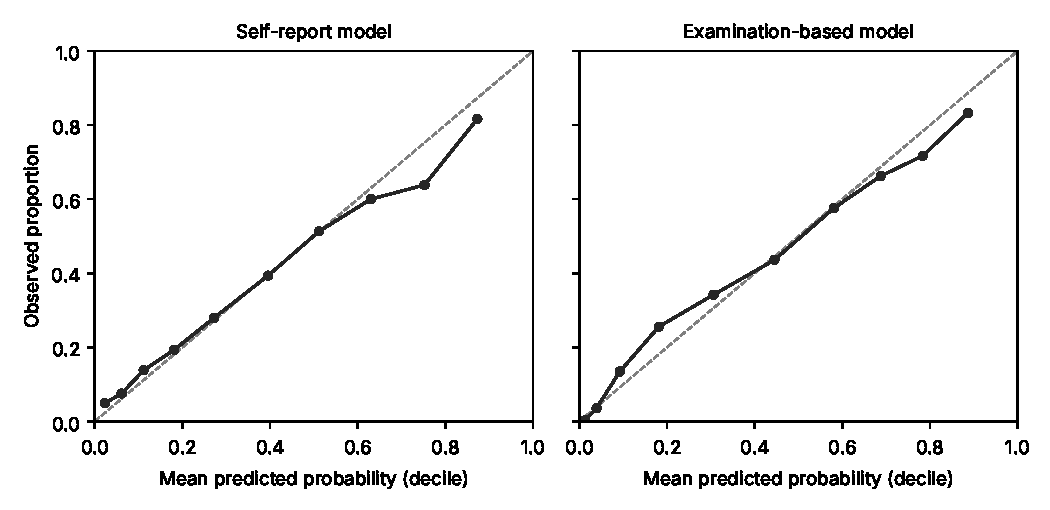
\includegraphics[width=\columnwidth]{figA1.pdf}\caption{Calibration of the models used to generate counterfactuals on the 2015–2018 test split (deciles of predicted probability; dashed line: perfect calibration). Post hoc reporting.}\end{figure}

\textbf{Data characteristics.} Table A.8 lists every feature with its
NHANES source, coding, distribution and missingness.

\begin{table*}[!htbp]
\caption{Features, coding, distribution and missingness of the analytic samples (unweighted).}
\label{tabA8}
\scriptsize\def\baselinestretch{1}\selectfont\renewcommand{\arraystretch}{1.1}
\begin{tabularx}{\textwidth}{>{\raggedright\arraybackslash}p{0.19\linewidth}>{\raggedright\arraybackslash}p{0.21\linewidth}>{\raggedright\arraybackslash}X>{\raggedright\arraybackslash}p{0.07\linewidth}>{\raggedright\arraybackslash}X>{\raggedright\arraybackslash}p{0.07\linewidth}}
\toprule
\textbf{Feature} & \textbf{NHANES source; coding} & \textbf{2011–2014, median [IQR] or \%} & \textbf{Missing, \%} & \textbf{2015–2018, median [IQR] or \%} & \textbf{Missing, \%} \\ \midrule
Age & RIDAGEYR; years & 49 [34; 63] & 0.0 & 51 [35; 65] & 0.0 \\
Female sex & RIAGENDR & 50.6\% & 0.0 & 51.1\% & 0.0 \\
Race/ethnicity, \% (6 indicators) & RIDRETH3 = 1 / 2 / 3 / 4 / 6 / 7 & 11.6 / 9.5 / 40.1 / 23.3 / 12.6 / 2.9 & 0.0 & 15.4 / 11.2 / 33.9 / 22.3 / 12.8 / 4.3 & 0.0 \\
Education & DMDEDUC2; 1-5 & 4 [3; 5] & 0.1 & 4 [3; 4] & 0.1 \\
Income-to-poverty ratio & INDFMPIR; ratio & 2.02 [1.03; 4.08] & 7.8 & 2.09 [1.15; 3.98] & 11.3 \\
Insured & HIQ011 & 77.6\% & 0.1 & 83.9\% & 0.2 \\
Usual place of care & HUQ030 & 84.2\% & 0.0 & 82.1\% & 0.0 \\
Visits in past year & HUQ051, HUQ050; category 0-8 & 2 [1; 3] & 0.1 & 2 [1; 3] & 0.2 \\
Cholesterol ever checked (not used) & BPQ060 & 64.2\% & 36.5 & 69.8\% & 38.0 \\
Told diabetes & DIQ010; 0/0.5/1 & 0 [0; 0] & 0.1 & 0 [0; 0] & 0.1 \\
Told high cholesterol & BPQ080 & 34.7\% & 0.6 & 35.5\% & 0.7 \\
Current smoker & SMQ020, SMQ040 & 20.4\% & 0.1 & 18.7\% & 0.1 \\
Drinks per drinking day & ALQ130 (+ALQ101, ALQ111); drinks/day & 1.0 [1.0; 3.0] & 19.3 & 2.0 [1.0; 3.0] & 21.4 \\
Vigorous recreational activity & PAQ650 & 22.3\% & 0.0 & 24.2\% & 0.0 \\
Moderate recreational activity & PAQ665 & 41.8\% & 0.0 & 40.7\% & 0.0 \\
BMI & BMXBMI; kg/m2 & 27.7 [24.0; 32.3] & 1.1 & 28.5 [24.7; 33.4] & 1.1 \\
Waist & BMXWAIST; cm & 97.2 [86.8; 108.3] & 4.9 & 99.1 [88.6; 110.5] & 5.0 \\
Total cholesterol & LBXTC; mg/dL (x0.02586 = mmol/L) & 188 [163; 216] & 5.6 & 186 [161; 214] & 5.7 \\
HbA1c & LBXGH; \% (NGSP) & 5.5 [5.2; 5.9] & 4.1 & 5.6 [5.3; 6.0] & 4.5 \\
Self-rated health & HUQ010; 1-5 (1 = excellent) & 3 [2; 3] & 0.1 & 3 [2; 4] & 0.1 \\
\bottomrule
\end{tabularx}
\par\vspace{2pt}{\scriptsize\raggedright Feature groups as in Section 2.2. RIDRETH3: 1 Mexican American, 2 Other Hispanic, 3 non-Hispanic White, 4 non-Hispanic Black, 6 non-Hispanic Asian, 7 other or multiracial. Missing \% differed by at most 1.4 percentage points between training and test splits. Skip patterns resolved by the feature builder: never smokers have current\_smoker = 0 and never drinkers have drinks\_per\_day = 0; BPQ060 is skipped when high cholesterol was reported and was dropped. Refused and don't-know codes were set to missing; no other outlier removal or truncation was applied. Class balance (positive \%): $Y_{\mathrm{self}}$ 37.0\% and $Y_{\mathrm{clin}}$ 36.5\% in 2011–2014; 37.8\% and 40.0\% in 2015–2018; no resampling or class weighting was used.\par}
\end{table*}

\textbf{Clinical translation roadmap (proposed, not evaluated).}
\emph{Intended users:} model developers, clinical informatics and AI
governance teams. \emph{Position in the workflow:} after model
development and before release of a CF-based decision support tool; PLCA
does not run at the point of care and produces no patient-facing output.
\emph{Current readiness:} technology readiness level 3--4, self-assessed
against the machine learning TRL framework {[}32{]} (analytical proof of
concept on public survey data). \emph{Steps before any deployment:} (1)
repeat the audit on electronic health record data with a diagnosis code
and measured blood pressure for the same patients; (2) clinician review
of the constraint rules and of a sample of CFs; (3) prespecified
acceptance criteria for valid-CF coverage and for A under each
constraint setting; (4) re-audit after model updates or data drift.
\emph{Not yet studied:} usability, effect on clinical decisions, and
patient outcomes.

\textbf{Computing environment.} All endpoint results: one run of
\url{scripts/run_all.sh} at commit 85a813b on a Linux laptop (Intel Core
i5-1335U, 16 GB RAM; Python 3.12.3, XGBoost 3.4.1, scikit-learn 1.9.1,
dice-ml 0.12). Package versions: \url{results/pip_freeze.txt};
environment: \url{results/environment.json}. Analysis code was written
with assistance from Claude (Anthropic); all code was reviewed and run
by the author, and every reported number is read from the output files
of these runs.

\end{document}
